\section{Results and discussion}

In this section we detail the findings of our study. We first present the results of each study
in Section~\ref{sec:res-fs} and Section~\ref{sec:res-ss}. In Section~\ref{sec:discussion} we summarize the
implications of our study. 

\subsection{Result of the first study: A non-exact replication}\label{sec:res-fs}

Our first study performed a replication of \blls.
%\kn{We should introduce an abbreviation for the Bao et al work and reuse it everywhere. What do you think? }. 
As discussed in the previous section, we first executed the analysis using the DroidXP benchmark with its default configuration. After that, we executed the analysis again by disabling the DroidFax static analysis algorithm, so that we could better estimate the performance of the dynamic analysis tools for mining Android sandboxes. Table~\ref{tab:fs} summarizes the results of the execution. The columns Exec. (WS) and Exec. (WOS) 
show the number of malwares identified when executing each tool with the
support of the DroidFax static analysis algorithms(WS) and without the support
of DroidFax static analysis algorithms(WOS). 
%\kn{I have changed the I and II to Ws and WOS because I and II makes it sound like we ran the experiments two times which we have not yet done. }
The Impact column shows the impact
(in percentage) of DroidFax static analysis algorithms in the results.
%\kn{Is this really improvement? Is this not "contribution" of droidfax. Improvement happens when an earlier approach detected malware without support of droidfax. Here 23\% of malwares are simply detected by the presence of droidfax (so IMO it should be impact or contribution) not improvement}
In the \blls, the authors do not present a
discussion about the influence of DroidFax in the results, even
though here we report that the impact of DroidFax to the results is significant in the
range from 16.44\% (DroidBot) to 51.79\% (Humanoid)---discarding our
\joke tool for which DroidFax improves its performance by 100\% (as expected).
Next we discuss the result of each individual test generation tool. 

\begin{table}[ht]
  \caption{Summary of the results of the first study. }
  \centering
  \begin{small}
 \begin{tabular}{lrrr}
   \toprule
   Tool & Exec. (WS) & Exec. (WOS) & Impact (\%) \\   \midrule
   DroidBot &  73 & 61 & 16.44 \\ 
   Monkey &  71 & 56 & 21.13 \\ 
   DroidMate &  68 & 52 & 23.53 \\ 
   Humanoid &  56 & 27 & 51.79 \\ 
\joke &  42 & 0 & 100.00 \\ 
 \bottomrule
 \end{tabular}
 \end{small}
 \label{tab:fs}
\end{table}


\subsubsection*{Monkey} sandbox for the execution WS detected in our study ($71$ out of the $96$ pairs of Android apps). Contrasting, in the original study, where Monkey got the third-best performance, detecting $48$ malwares within the 102 pairs ($47.05$\%). This difference might be due to the Monkey using strategy that incorporates randomness for test case generation. %\rb{I am not convinced that the other tools do not employ any randomness.} 
For our second execution (Exec WOS), there is a reduction of $21.13$\% in the Monkey's performance, totaling $56$ malware detected. %\rb{Considering only one run for each configuration, that is Exec. (I) and Exec. (II), we cannot assure that the difference is due to disabling the DroidFax static analysis algorithms.}


\subsubsection*{DroidBot} in the first execution (Exec. WS) its resulting sandbox detected a total of $73$ malware among $96$ pairs analyzed ($76.04$\%), more apps with malicious behavior than any other tool. Like the original study, DroidBot was the test case generation tool whose resulting sandbox detected the largest number of malicious apps. However, in our second execution (Exec WOS), its performance decreased to ($16.44$\%). %\rb{Not sure if the following sentence is right.} 
Despite this reduction, it detected the largest number of malicious apps in the Exec. WOS.

\subsubsection*{DroidMate} in the first execution(WS) led to a sandbox that detected 68 apps with malicious behavior ($70.83$\%). Contrasting, in the original study DroidMate detected $54$ among $102$ ($52.94$\%). A possible explanation for this difference is that here we use the more recent version of DroidMate. In the second execution(WOS), without the DroidFax static analysis algorithms, the resulting sandbox's performance drops by ($23.53$\%), being able to detect only 52 out of the 96 pairs of Android apps. 


\subsubsection*{Humanoid} presented the worse performance, even though a previous
work~\cite{DBLP:conf/kbse/LiY0C19} shows that it presents the highest lines coverage in comparison to Monkey, DroidBot, and DroidMate. In the first execution (WS), the resulting Humanoid sandbox identified $56$ malwares in our dataset ($58.33$\%). Since \blls did not explored Humanoid in their study, we do not have a baseline for comparison. Regarding the second execution, without static analysis, Humanoid was the most affected by disabling the DroidFax static analysis algorithm, losing ($51.79$\%) of its effectiveness, and being able to detect just $27$ malwares.

\subsubsection*{\joke} is our fake test case generation tool that we use to help us understand the performance of the DroidFax static analysis algorithm for mining sandboxes. We integrated \joke into the DroidXP benchmark as an additional test generation tool that does not run the Android apps during the benchmark execution. As a result, the analysis using \joke reveals the performance of DroidFax static analysis algorithms only. For the first execution, with the DroidFax static algorithms enabled, even though \joke does not execute the Android apps, its resulting sandbox detected 43.75\% of the malwares. For the second execution, that is, disabling the DroidFax static analysis algorithm, the resulting \joke sandbox was unable to detect any malware. This result was expected, since \joke does not analyze the Android apps during the benchmark execution.

\begin{finding}
  Integrating the dynamic analysis tools
  with the DroidFax static analysis algorithms
  improves substantially the performance
  of the resulting Android sandboxes for
  detecting malicious behavior. 
\end{finding}
 
The Venn-diagram of Figure~\ref{fig:venn-plot1}
summarizes how the tools can complement each other.
Note in the diagram that $53$ malwares have been detected by all sandboxes generated in the first execution (with the DroidFax static analysis algorithms), out of the 78 identified by at least one sandbox. In addition, the DroidBot sandbox did not detect any malware that had not been detected by the other tools. Differently, the Monkey's sandbox detected three malwares that had not been detected by any other sandbox, DroidBot sandbox detected two malwares that had not been detected by any other sandbox, and Humanoid detected one malware that had not been detected by any other sandbox. Contrasting with the \blls,
our results suggest that using DroidBot in combination with Monkey, DroidMate, and Humanoid does not improve the general performance of an integrated environment for mining
Android sandboxes.

\begin{finding}
  Our results suggest that one might benefit from using  an integrated
  environment that combines Monkey, DroidMate, and Humanoid to
  mine Android sandboxes. Introducing the DroidBot 
  tool does not improve the results.
\end{finding}


\begin{figure}[htb]
  \centering{
  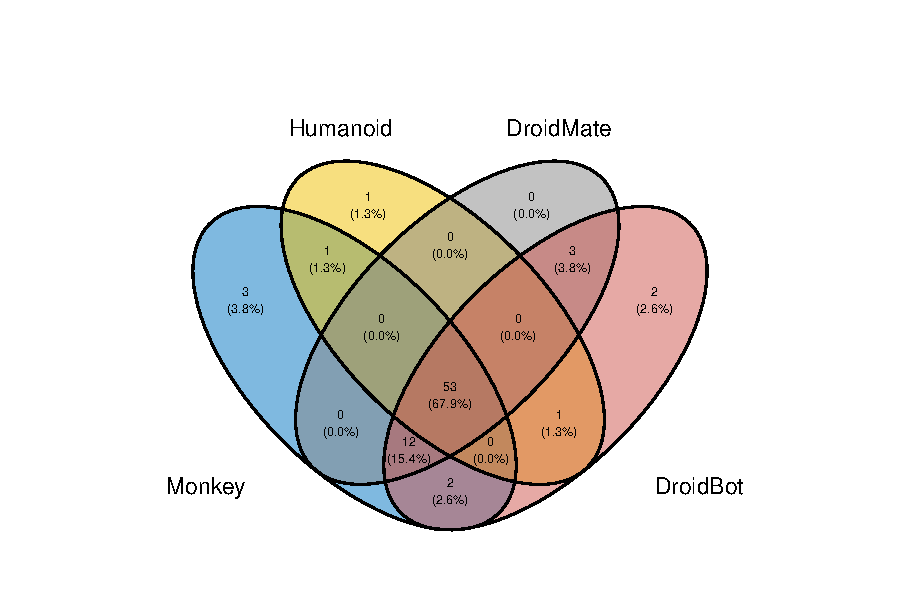
\includegraphics[trim=60 20 0 50,scale=0.7]{images/venn-plot-s1-1.pdf}}
  \caption{Venn Diagram highlighting how the sandboxes from the tools can
    complement each other.}
  \label{fig:venn-plot1}
\end{figure}


Altogether, ignoring the \joke tool, our study reveals that from $58.33$\% (Humanoid)
to $76.04$\% (DroidBot) of the malicious apps investigated in our study can be
detected using the sandboxes generated after running the test case tools with the support of DroidFax static analysis algorithms. Besides that, in the first execution, none of the resulting sandboxes could detect 18 malwares in our dataset ($18.75$\%). According to the Euphony tool~\cite{hurier2017euphony}, $12$ of these $18$ malwares are \emph{adwares}, $3$ are \emph{trojans}, $2$ are PUPs (\emph{Potentially Unwanted Program}), and one is an \emph{exploit}. In what follows we present some characteristics of two malware that had not been detected by the sandboxes (mobi.infolife.cachepro) and (com.andoop.flyracing), both downloaded from alternative android market, anzhi~\cite{anzhi}.

The first listing refers to package (mobi.infolife.cachepro), which has a less dangerous malicious strategies, and just translate the app from English language to Chinese language. That modification, does not threaten the user's device, however it is a unwanted private app change, and can characterize as misappropriation app.

\begin{lstlisting}[caption= smali/mobi/infolife/cachepro/h.smali - (mobi.infolife.cachepro),language=Java, basicstyle=\fontsize{8}{6}\selectfont\ttfamily,label={lst:mobi.infolife.cachepro}]

1:B < const-string v3, "Swith To "
---
1:M > const-string v3, "\u65e0\u6cd5\u542f\u52a8\u5e94\u7528\u201c"
\end{lstlisting}

\begin{lstlisting}[caption=AndroidManifest.xml - (com.andoop.flyracing), language=Java, basicstyle=\fontsize{8}{6}\selectfont\ttfamily,label={lst:app65}]

1:B < <meta-data android:name="ADMOB_PUBLISHER_ID"
                     android:value="a14cf7346295891"/>
---
1:M > <meta-data android:name="ADMOB_PUBLISHER_ID"
                     android:value="a14f099bfbf3c61"/>
\end{lstlisting}


The second listing refers to package (com.andoop.flyracing). Your malicious version change the Android Manifest file, modifying the identification of meta-data ADMOB\_PUBLISHER\_ID. AdMob \cite{admob} is a mobile app monetization service, provided by Google. The Publisher ID \cite{publisherID} is the unique identifier for the AdMob account, and may be used to authenticate communication with Google. With that change, the malware is changing the ad revenue destination. 

Now we present an malicious app that was detected by 2 sandboxes. The package (com.gau.screenguru.finger) belongs to ours dataset, and is a troubling example. First it modify the Android Manifest file, adding permissions to receive and send SMS (Listing 3). Then, the malicious app use those permissions to performs MainService.java file, that get user's sensitive information, like International Mobile Equipment Identity (IMEI), and sink by SMS message (Listing 4). This malicious behaviours was detected by sandboxes builded by Droidbot and Humanoid tools.

\begin{lstlisting}[caption= AndroidManifest.xml - (com.gau.screenguru.finger), language=Java, basicstyle=\fontsize{8}{6}\selectfont\ttfamily,label={lst:com.gau.screenguru.finger:androidmanifest}]

67:M >    <uses-permission android:name="android.permission.RECEIVE_SMS"/>
68:M >    <uses-permission android:name="android.permission.SEND_SMS"/>
\end{lstlisting}

\begin{lstlisting}[caption= com/android/main/MainService.java - (com.gau.screenguru.finger), language=Java, basicstyle=\fontsize{8}{6}\selectfont\ttfamily,label={lst:(com.gau.screenguru.finger):mainservice}]

492:M > localObject2 = (TelephonyManager)getSystemService("phone");
493:M > if (localObject2 != null)
494:M > {
495:M >  this.imei = ((TelephonyManager)localObject2).getDeviceId();
496:M >  this.imsi = ((TelephonyManager)localObject2).getSubscriberId();
497:M >  this.iccid = ((TelephonyManager)localObject2).getSimSerialNumber();
498:M > }
// [...]
519:M > if ("".equals(this.destMobile)) {
520:M >  getDestMobile();
521:M > }
522:M > sendSMS(this.destMobile, "imei:" + this.imei)
\end{lstlisting}



%\rb{This is an interesting place to present the details of two or three malwares in this set of 19 malwares that had not been detected by any tool. I think Thales could work on this, since he has helped Handrick to dissect the malwares.}

\subsection{Result of the second study: Tainted analysis algorithms.}\label{sec:res-ss}

In this second study we used a tainted analysis approach to mine differences between the benign and malicious versions of each of the 96 Android apps in our dataset. To this end we leverage the FlowDroid tool, which tracks how sensitive information flows through the apps using tainted analysis algorithms. Regarding accuracy, the tainted analysis approach detected $58$ out of the $96$ pairs in our dataset ($60,42$\%), that is, the FlowDroid approach leads to a better performance than any sandbox originated in the second execution of the dynamic analysis tools (without the DroidFax static analysis algorithms).

\begin{finding}
  The performance of FlowDroid to identify malicious behavior
  is superior than the performance of the
  mining sandbox approach supported by dynamic analysis only---without
  the DroidFax static analysis algorithms.
\end{finding}

Additionally, we investigate if we could benefit from combining
the results from FlowDroid and DroidFax. Figure~\ref{fig:venn-plot2} shows a
Venn-diagram summarizing the results. So, when combining
the results from FlowDroid and DroidFax, we were able to detect
$67$ of the malicious apps ($69.79$\%), a performance compatible
to that we found as response to the first execution of the
test case generation tools---which also considers the DroidFax
static analysis algorithms. More interesting, from those $67$
malicious apps identified, $33$ pairs had been found by
both tools (FlowDroid and DroidFax), even though they follow
a completely different static analysis approach. Furthermore,
FlowDroid shows to be more effective than DroidFax, detecting $25$ malicious
apps that had not been detected by DroidFax (while DroidFax detected $9$
malicious apps that had not been detected by FlowDroid).

\begin{finding}
  Integrating the results of static analysis tools
  (such as FlowDroid and DroidFax) seems promising,
  leading to a performance similar to that achievend
  when combining test case generation tools with the
  DroidFax tool. 
\end{finding}

\begin{figure}
  \centering{
  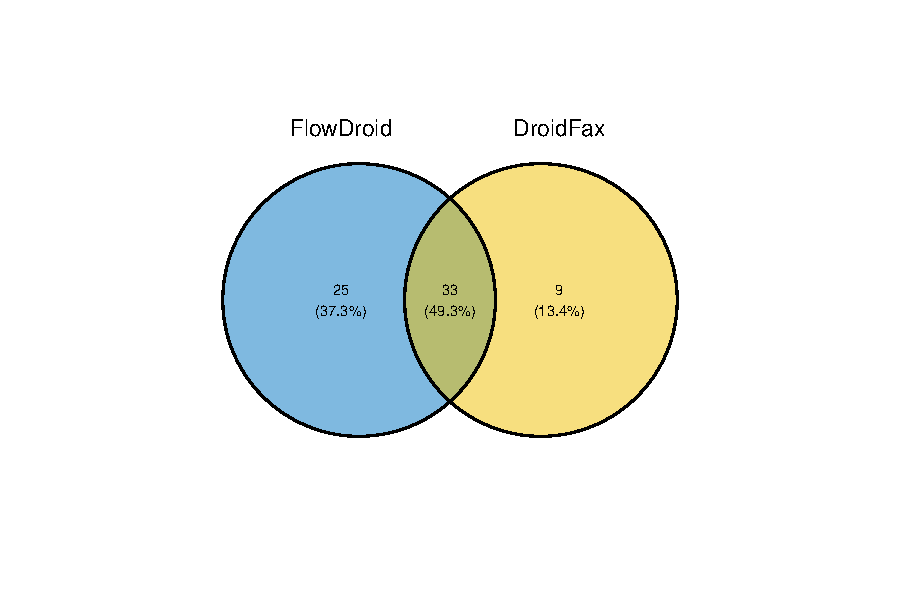
\includegraphics[trim=60 20 0 50,scale=0.7]{images/venn-plot-s2-1.pdf}}
  \caption{Venn Diagram highlighting the possible benefits of
    integrating FlowDroid and DroidFax.}
  \label{fig:venn-plot2}

\end{figure}

The execution of FlowDroid is also feasible: the analysis takes only
32.08 seconds per app on average, totaling a processing time of 52
minutes to analyze all 96 pairs of Android apps.
Even though the time to execute the FlowDroid analysis depends on the size
of the app, the longest run took only 437 seconds. 

Finally, we can highlight that FlowDroid was able to detect $4$ malwares among the $18$ malicious Android apps that had not
been detected by the sandboxes constructed in the first study. Among these
four malwares, $2$ are \emph{trojans}, $1$ is an \emph{exploit}, and 1 is an \emph{adware}.

\begin{finding}
  Although FlowDroid presents a performance similar
  to that of using the dynamic analysis approach for mining sandboxes,
  it was able to detect only four additional malwares (out of the
  18) that had not been detected in the first study. 
\end{finding}

Here we present details about one of the malware that Flowdroid had detected. At this package (com.yy.fontmaster), from another alternative android market, angeeks~\cite{angeeks}, the malicious and benign apps have the same sink, however they access different sources, therefore configuring additional source-sink pairs, and hence a possible malicious behaviours. The Figure \ref{fig:sourcesink}, presents the paths source (blue border) and sink (orange border) from benign and malicious apps.

\begin{figure}[ht]%
    \centering
    \subfloat[\centering Path source/sink from benign app]{{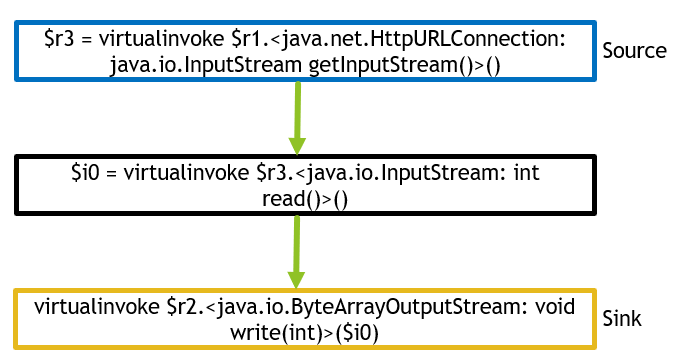
\includegraphics[width=5cm]{images/pathbenign.png} }}%
    \qquad
    \subfloat[\centering Path source/sink from malicious app]{{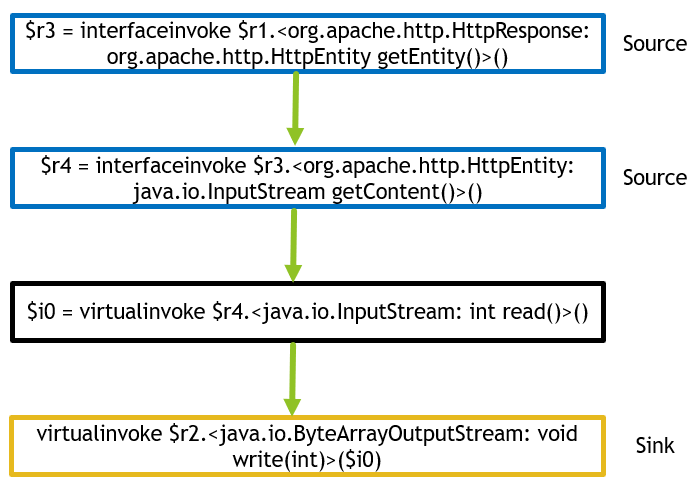
\includegraphics[width=5cm]{images/pathmalicious.png} }}%
    \caption{Pairs source/sink different (B/M)}%
    \label{fig:sourcesink}%
\end{figure}

\subsection{Discussion}\label{sec:discussion}

First we find that static analysis summaries had impact in the Bao et al. study. It was responsible for improving the results of the tools by 47.78\% than its executions alone, answering our first research question (RQ1). Second, Table \ref{tab:malwareWithout} summarizes our findings addressing the second research question (RQ2). We realized that disregarding the static analysis algorithms, and discarding Joke tool, among the tools analyzed in your study, Humanoid had the biggest performance drop, and the least affected was DroidBot, proving be the tool with better effective performance, in terms of the number of detected malware. Finally, we answered our last research question (RQ3) when we leverage sandboxes, complementing the dynamic analysis provided by test generation tool with tainted analysis algorithms. Our experiment highlight that 69.79\%-81.25\% of malware in dataset can be now uncovered by the complement of tainted analysis algorithms, evidencing that 
sandboxes can be further boosted when coupled with new static analysis techniques. We found that the number of identified malicious apps detected is increased for all cases, achieving at the best case, 81.25\% with Monkey, a better performance than all five tools explored at Bao et al., even when they combined all the tools together at theirs work 75.49\%. Table \ref{tab:tanted} display the increase of all tools explored at our research.

\begin{table}[ht]
\centering
\begin{tabular}{lccc}\toprule
 Test Generation & FlowDroid & Total & \%\\
 Tool & Increase  &  & \\ \midrule
 Monkey & 7 & 78 & 81.25\\
 DroidMate & 10 &  74 & 77.08 \\
 Humanoid & 20 & 69 & 71.87  \\
 Joke & 25 & 67 & 69.79 \\
 DroidBot & 9 & 77 & 80.20  \\\midrule
 
\end{tabular} 
\caption{Malwares detected in 96 pair (B/M) increased by Tainted analysis Algorithms}
\label{tab:tanted}
\end{table}


%%here we also have to write about the intersection between droidfax and tainted analysis now, and about what 1 reveled and other dont, and otherwise. 


%Here we can write about MOTIVATION EXAMPLES.
